%%%%%%%%%%%%%%%%%%%%%%%%%%%%%%%%%%%%%%%%%
% a0poster Portrait Poster
% LaTeX Template
% Version 1.0 (22/06/13)
%
% The a0poster class was created by:
% Gerlinde Kettl and Matthias Weiser (tex@kettl.de)
% 
% This template has been downloaded from:
% http://www.LaTeXTemplates.com
%
% License:
% CC BY-NC-SA 3.0 (http://creativecommons.org/licenses/by-nc-sa/3.0/)
%
%%%%%%%%%%%%%%%%%%%%%%%%%%%%%%%%%%%%%%%%%

%----------------------------------------------------------------------------------------
%	PACKAGES AND OTHER DOCUMENT CONFIGURATIONS
%----------------------------------------------------------------------------------------

\documentclass[a0,portrait]{a0poster}
\usepackage{multicol} % This is so we can have multiple columns of text side-by-side
\columnsep=100pt % This is the amount of white space between the columns in the poster
\columnseprule=3pt % This is the thickness of the black line between the columns in the poster

\usepackage[svgnames]{xcolor} % Specify colors by their 'svgnames', for a full list of all colors available see here: http://www.latextemplates.com/svgnames-colors

\usepackage{times} % Use the times font

\usepackage{graphicx} % Required for including images
\graphicspath{{FigJar/}} % Location of the graphics files
\usepackage{booktabs} % Top and bottom rules for table
\usepackage[font=small,labelfont=bf]{caption} % Required for specifying captions to tables and figures
\usepackage{amsfonts, amsmath, amsthm, amssymb} % For math fonts, symbols and environments
\usepackage{wrapfig} % Allows wrapping text around tables and figures
\usepackage{subcaption}
\usepackage{framed}

\begin{document}

%----------------------------------------------------------------------------------------
%	POSTER HEADER 
%----------------------------------------------------------------------------------------

% The header is divided into two boxes:
% The first is 75% wide and houses the title, subtitle, names, university/organization and contact information
% The second is 25% wide and houses a logo for your university/organization or a photo of you
% The widths of these boxes can be easily edited to accommodate your content as you see fit

\begin{minipage}[b]{0.75\linewidth}
\veryHuge \color{NavyBlue} \textbf{Derivation of Marine Inherent Optical Properties}
\Huge \color{Black} \textit{A Bayesian Approach}\\[2cm] % Subtitle
\huge \textbf{Erdem M. Karak{\"o}yl{\"u} \& Susanne E. Craig}\\[0.5cm] % Author(s)
\huge NASA Ocean Biology Processing Group\\[0.4cm] % University/organization
\Large \texttt{erdem.m.karakoylu@nasa.gov} --- (301) 286-0501\\
\end{minipage}
%
%\begin{minipage}[b]{0.25\linewidth}
%
\includegraphics[width=20cm]{logo.png}\\
%\end{minipage}
\begin{multicols}{2}
%----------------------------------------------------------------------------------------
%	INTRODUCTION
%----------------------------------------------------------------------------------------

\color{SaddleBrown} % SaddleBrown color for the introduction

\section*{Introduction}

The advent of satellite oceanography has generated tremendous incite in our understanding of global biogeophysical processes in the ocean by providing a synoptic view of phytoplankton distribution dynamics. One of the principle obstacles in this endeavor is the signal contributed to the sensed light field by the atmosphere. Some of this contribution, such as Rayleigh scattering, is straightforward to correct for. However, light contribution by spatio-temporally  variable aerosol distribution has so far been addressed by removing a modelled approximation of its contribution to estimate the water signal. This works  well in the open ocean, but runs into trouble in coastal regions, where both marine and atmospheric layers are often optically complex. 

Here, we propose circumventing the atmospheric complexity of coastal areas by using \textbf{top-of-the-atmosphere radiance (TOA)} as indirect model input. We develop, and compare alternative models to estimate \textbf{phytoplankton absorption (aph)} - a proxy for phytoplankton distribution - using a bayesian modeling framework.

%----------------------------------------------------------------------------------------
%	OBJECTIVES
%----------------------------------------------------------------------------------------

\color{DarkSlateGray} % DarkSlateGray color for the rest of the content

\section*{Objectives}

\begin{enumerate}
    \item Estimate \textbf{aph} at 6 spectral bands from \textbf{TOA}.
    \item Develop feature-selecting \underline{\emph{Bayesian linear and nonlinear models}}.
    \item Use performance assessment and information theory for evaluation and model selection.
\end{enumerate}
%----------------------------------------------------------------------------------------
%	MATERIALS AND METHODS
%----------------------------------------------------------------------------------------

\section*{Materials and Methods}
Three models were developed:
\begin{enumerate}
    \item Linear regression with regularized horseshoe  (\textbf{RHS}) prior\cite{Vehtari:2017b}; hereafter, \textbf{Model 1}.
    \item Linear regression with \textbf{rHSP} and $1^{st}$ order feature interactions; hereafter, \textbf{Model 2}.
    \item Bayesian neural network \cite{Neal:1996bnn}; hereafter, \textbf{Model 3}.
\end{enumerate}

%------------------------------------------------

\subsection*{Model Development}
\begin{center}\vspace{1cm}
  \fbox{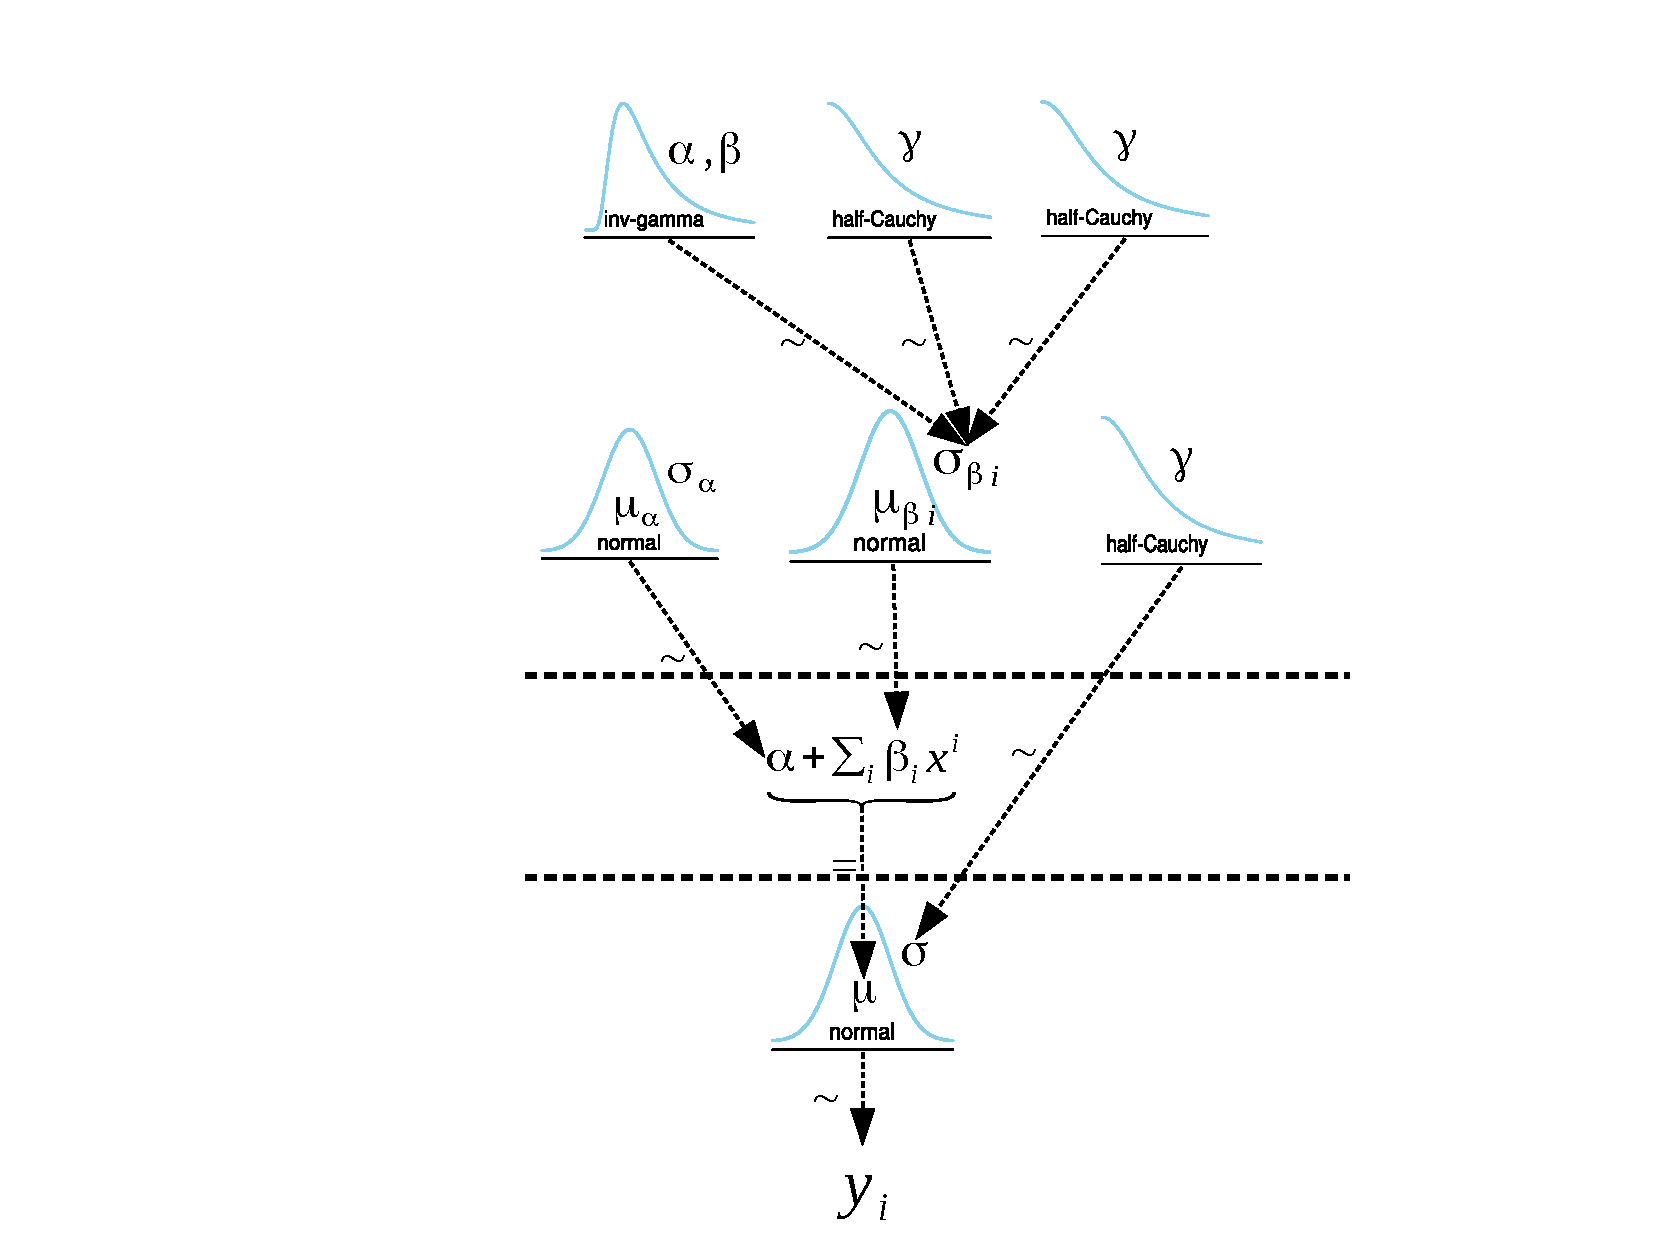
\includegraphics[trim={6cm 0cm 3cm 0cm}, clip=true, height=16cm, width=0.40\columnwidth]{krusche_diagrams_hs_reg}\hfill}
  \fbox{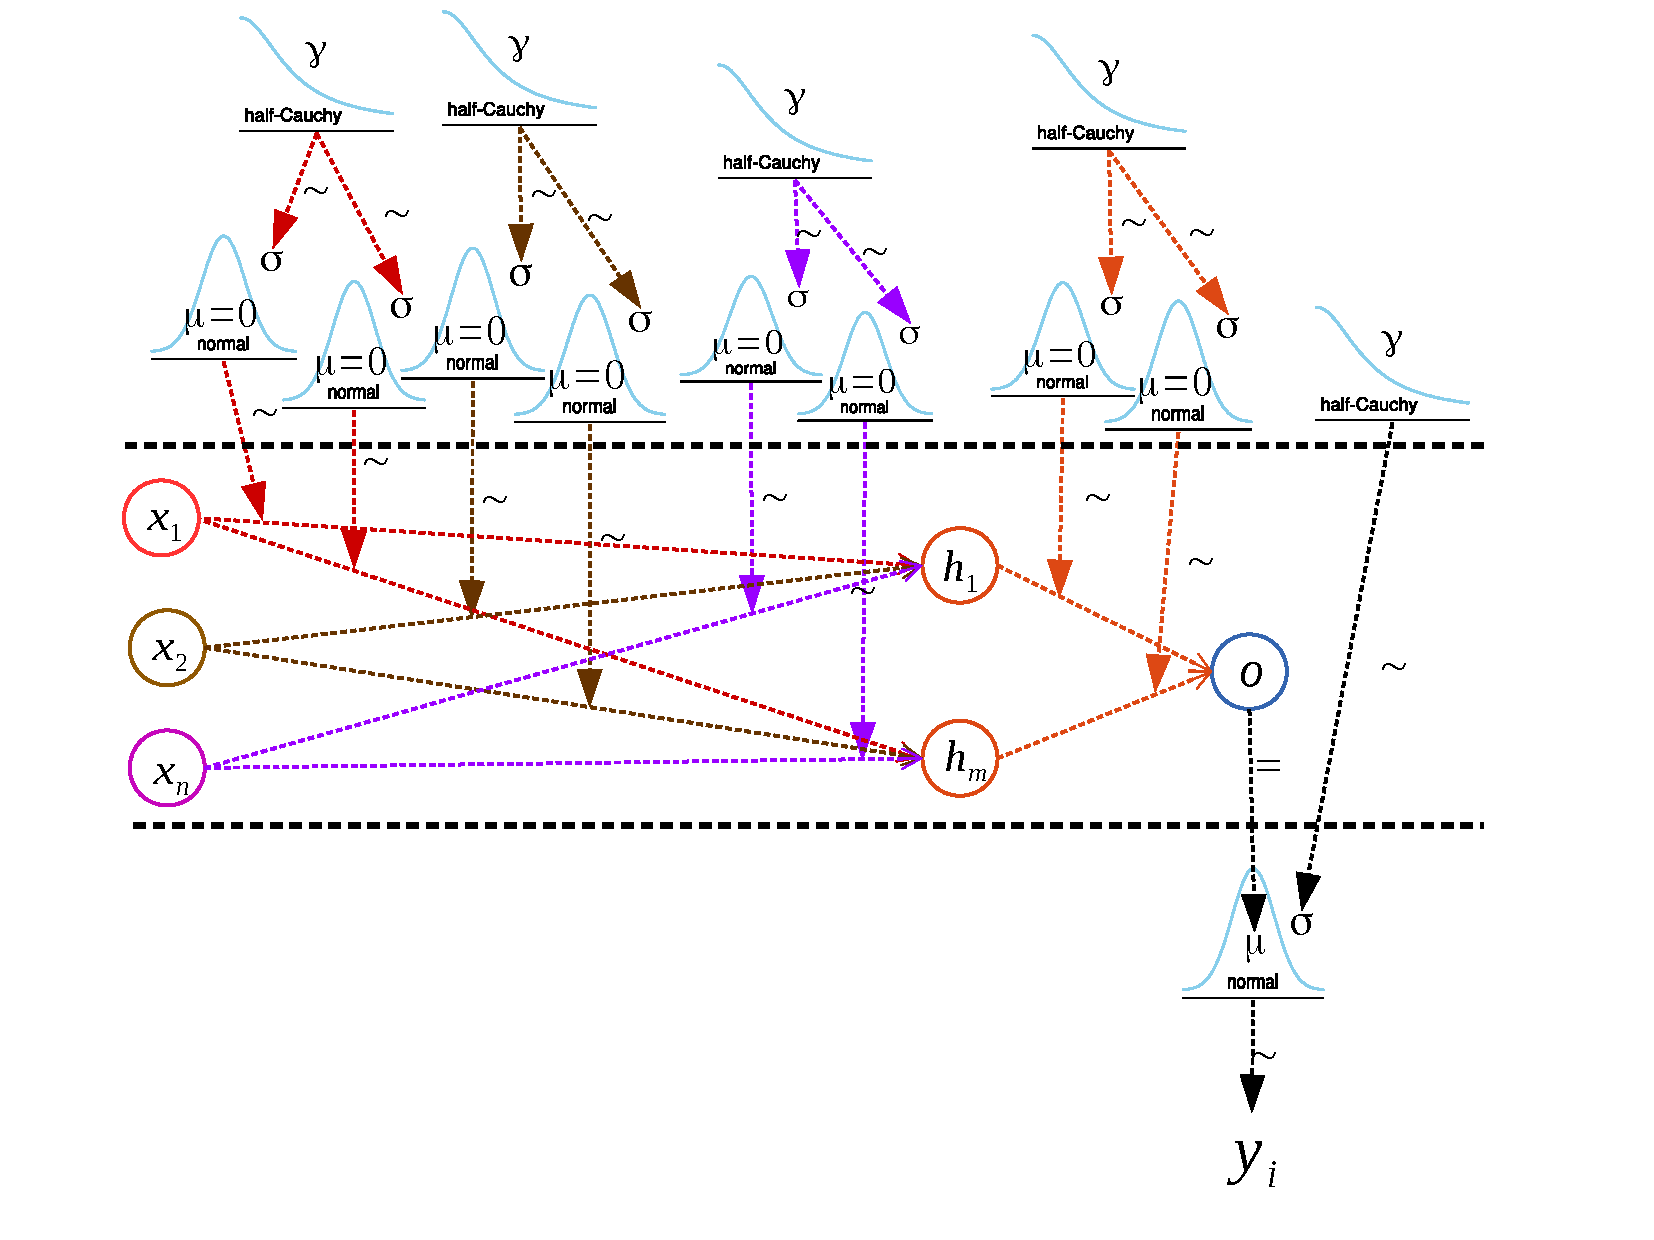
\includegraphics[trim={1cm 0cm 1.5cm 0cm}, clip=true, height=16cm, width=0.58\columnwidth]{krusche_diagrams_BNN}\hfill}
  \captionof{figure}{Inference diagram of Bayesian models used. Horizontal lines separate three conceptual groups; top $\rightarrow$ priors, middle $\rightarrow$ likelihood, bottom $\rightarrow$ outcome distribution. \textbf{Left:} Regression with horseshoe priors (Models 1 \& 2). \textbf{Right:} Bayesian neural network (Model 3). Models shown here are hierarchical, built for automatic feature relevance determination.} 
\end{center}


\subsection*{Data Pre-Processing}
Data consisted in satellite/in-situ data matchups as in \cite{Bailey:06}, where TOA radiance was matched to in-situ measured phytoplankton absorption at 6 wavelengths; 411, 443, 489, 510, 555, and 670 nm. Pre-processing highlights: \textbf{(1)} principle components (\textbf{PC}) computed from correlated TOA radiance; \textbf{(2)} features include PCs, water temperature (\textbf{SST}), solar zenith angle (\textbf{SolZ}), depth (\textbf{Bathy}); \textbf{(3)} though not strictly required in a Bayesian setting, data was split into training/testing (out-of-sample) sets.
%\begin{enumerate}
%    \item Computation of Principle Components (PC) from correlated TOA radiance data.
%    \item Features include PCs, water temperature, solar zenith angle, bathymetry.
%    \item Though not strictly required in a Bayesian setting, data was split into training/testing sets.
%\end{enumerate}
%\end{center}\vspace{1cm}
\begin{center}
    \fbox{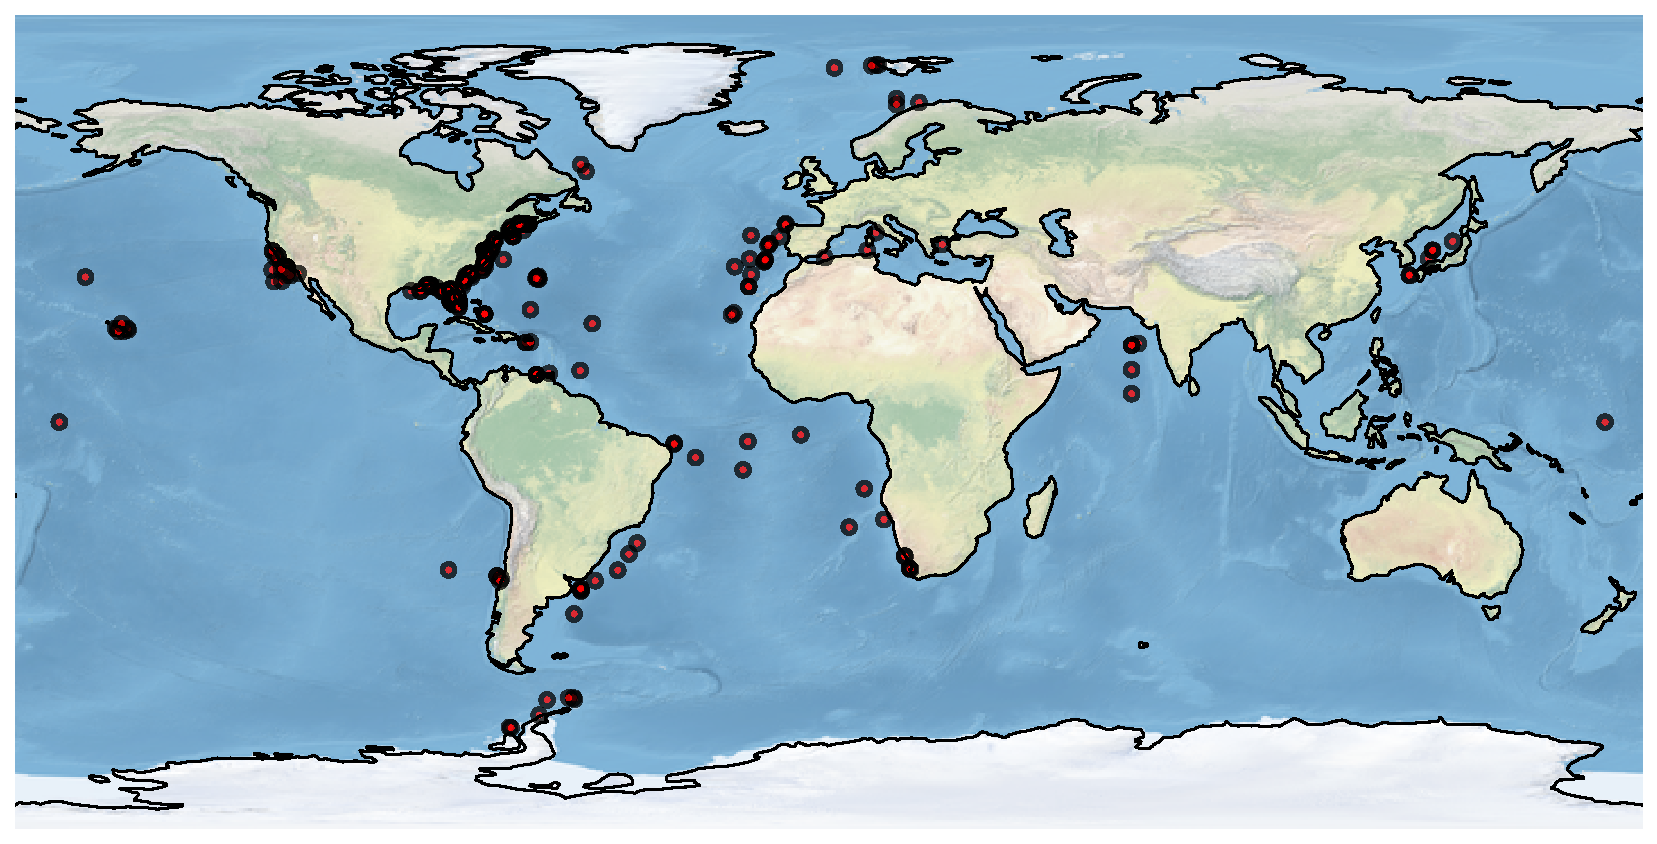
\includegraphics[height=13.6cm, width=0.56\linewidth]{map}
    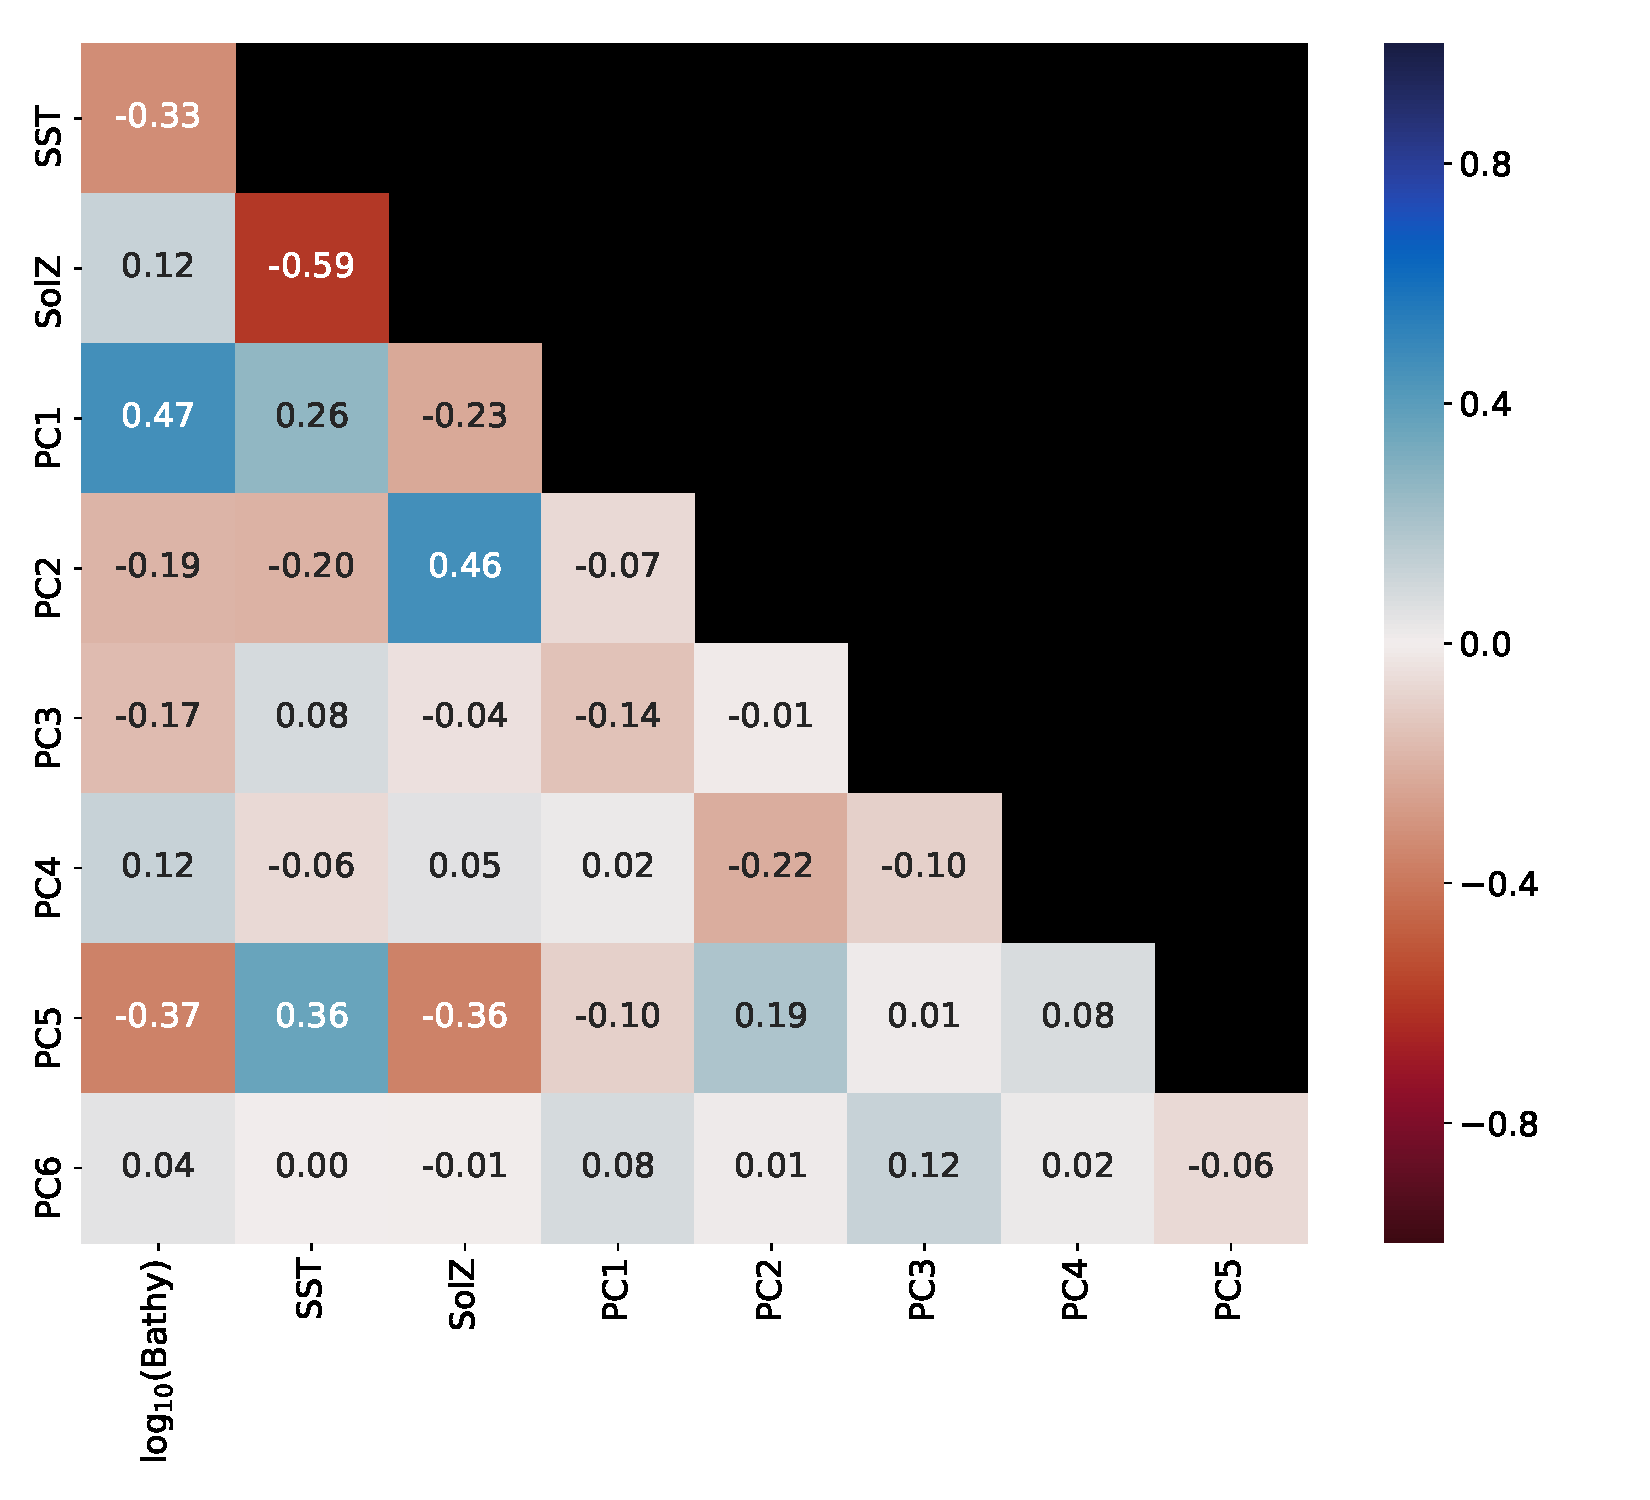
\includegraphics[width=0.43\linewidth]{feature_pairwise_map_notarget}}
    \captionof{figure}{\textbf{Left}: in-situ sampling locations are mostly coastal; continental or insular. \textbf{Right}: Features used in all models.}
\end{center}
%----------------------------------------------------------------------------------------
%	RESULTS 
%----------------------------------------------------------------------------------------

\section*{Results}
\begin{center}\vspace{1cm}
  \fbox{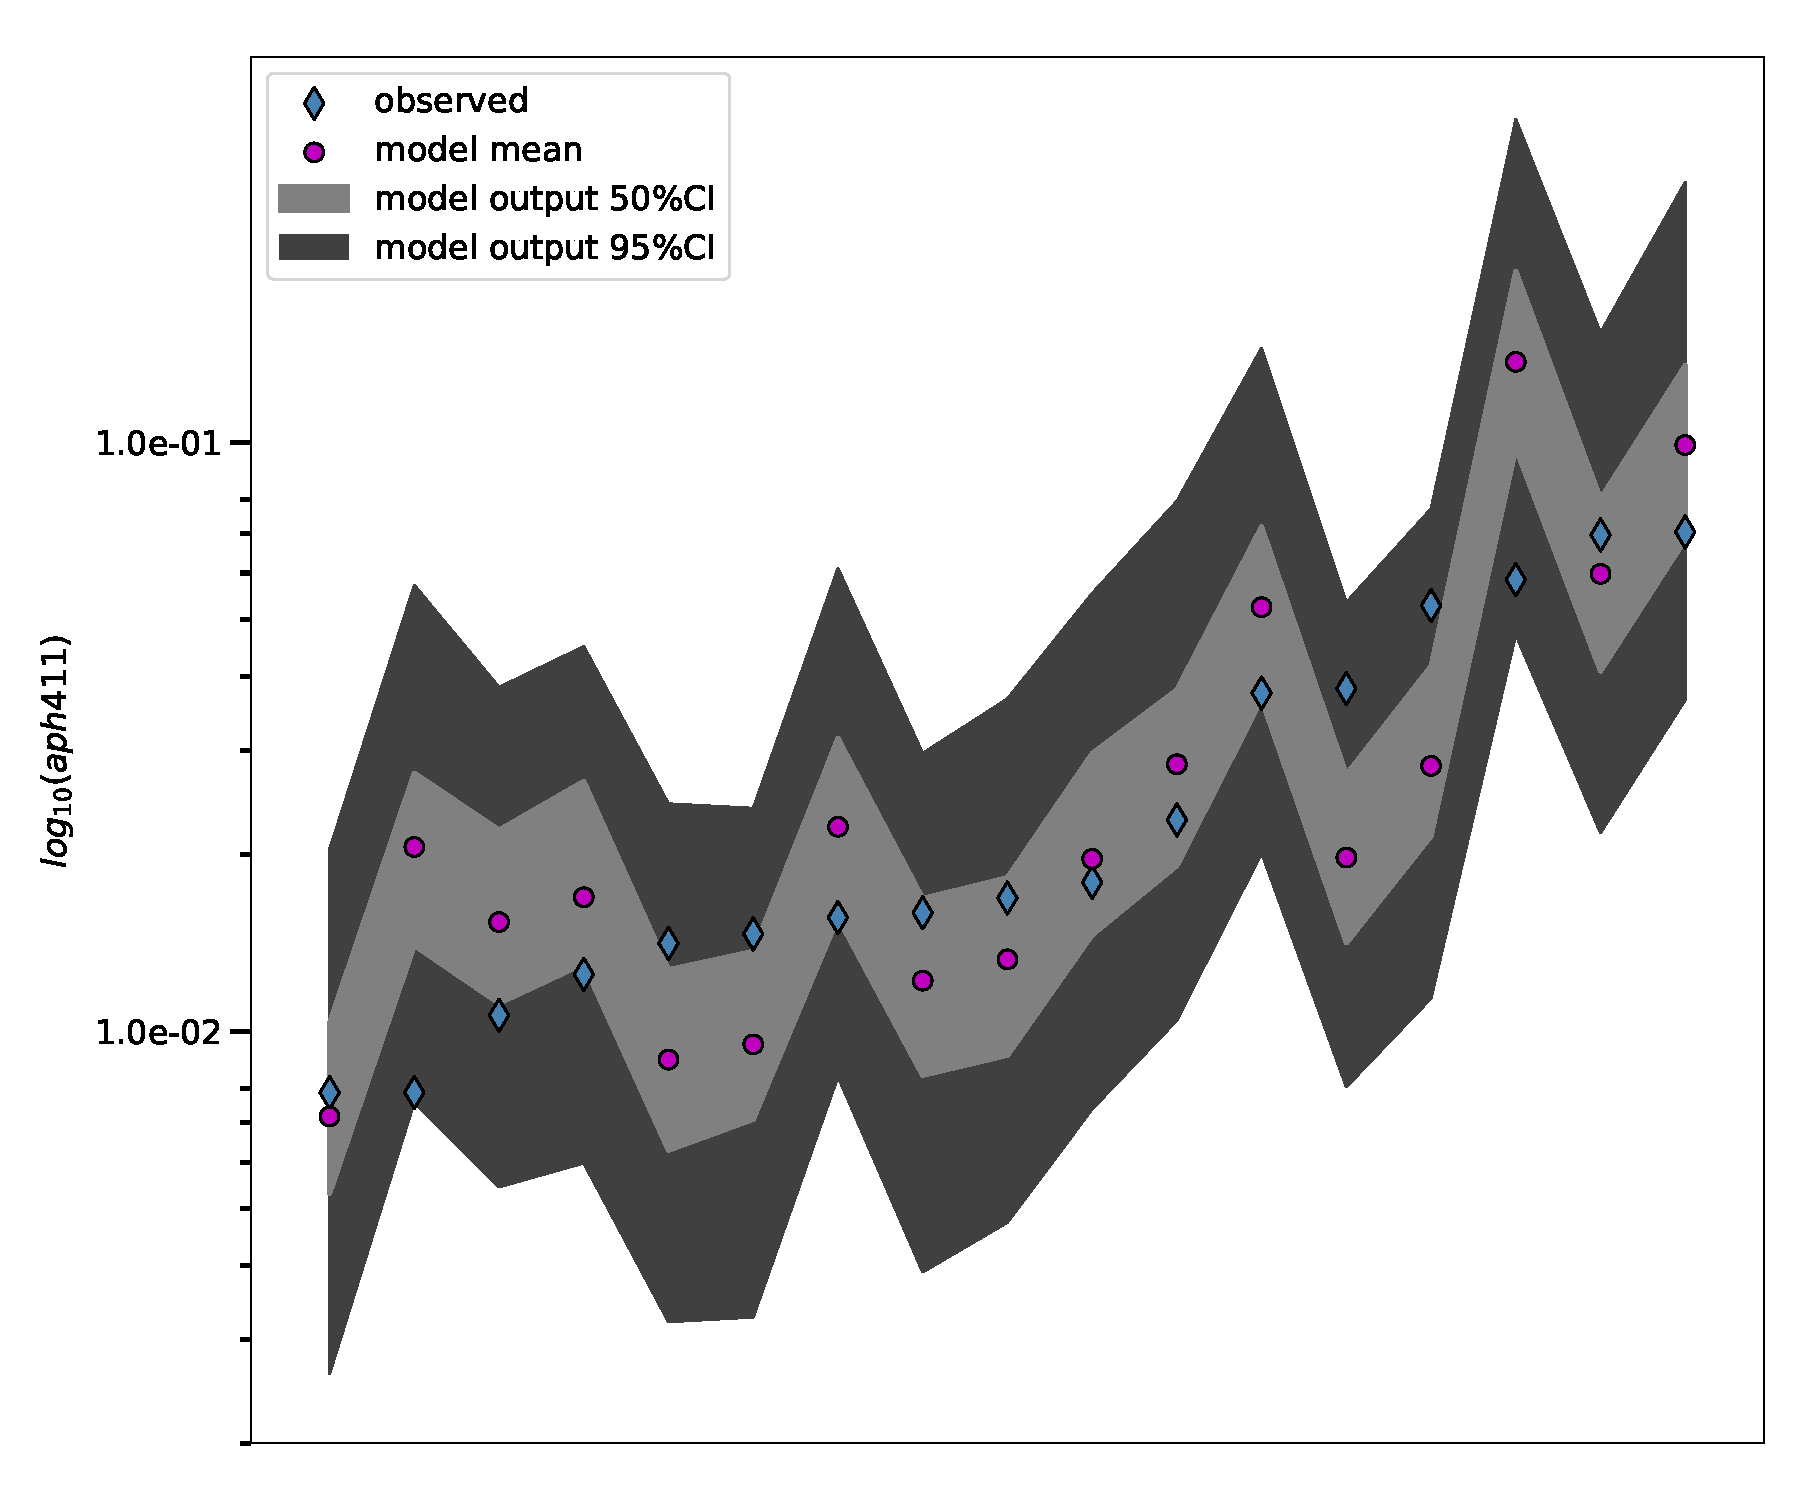
\includegraphics[height=15cm, width=0.55\columnwidth]{ppc_1_hs_aphi_411}
  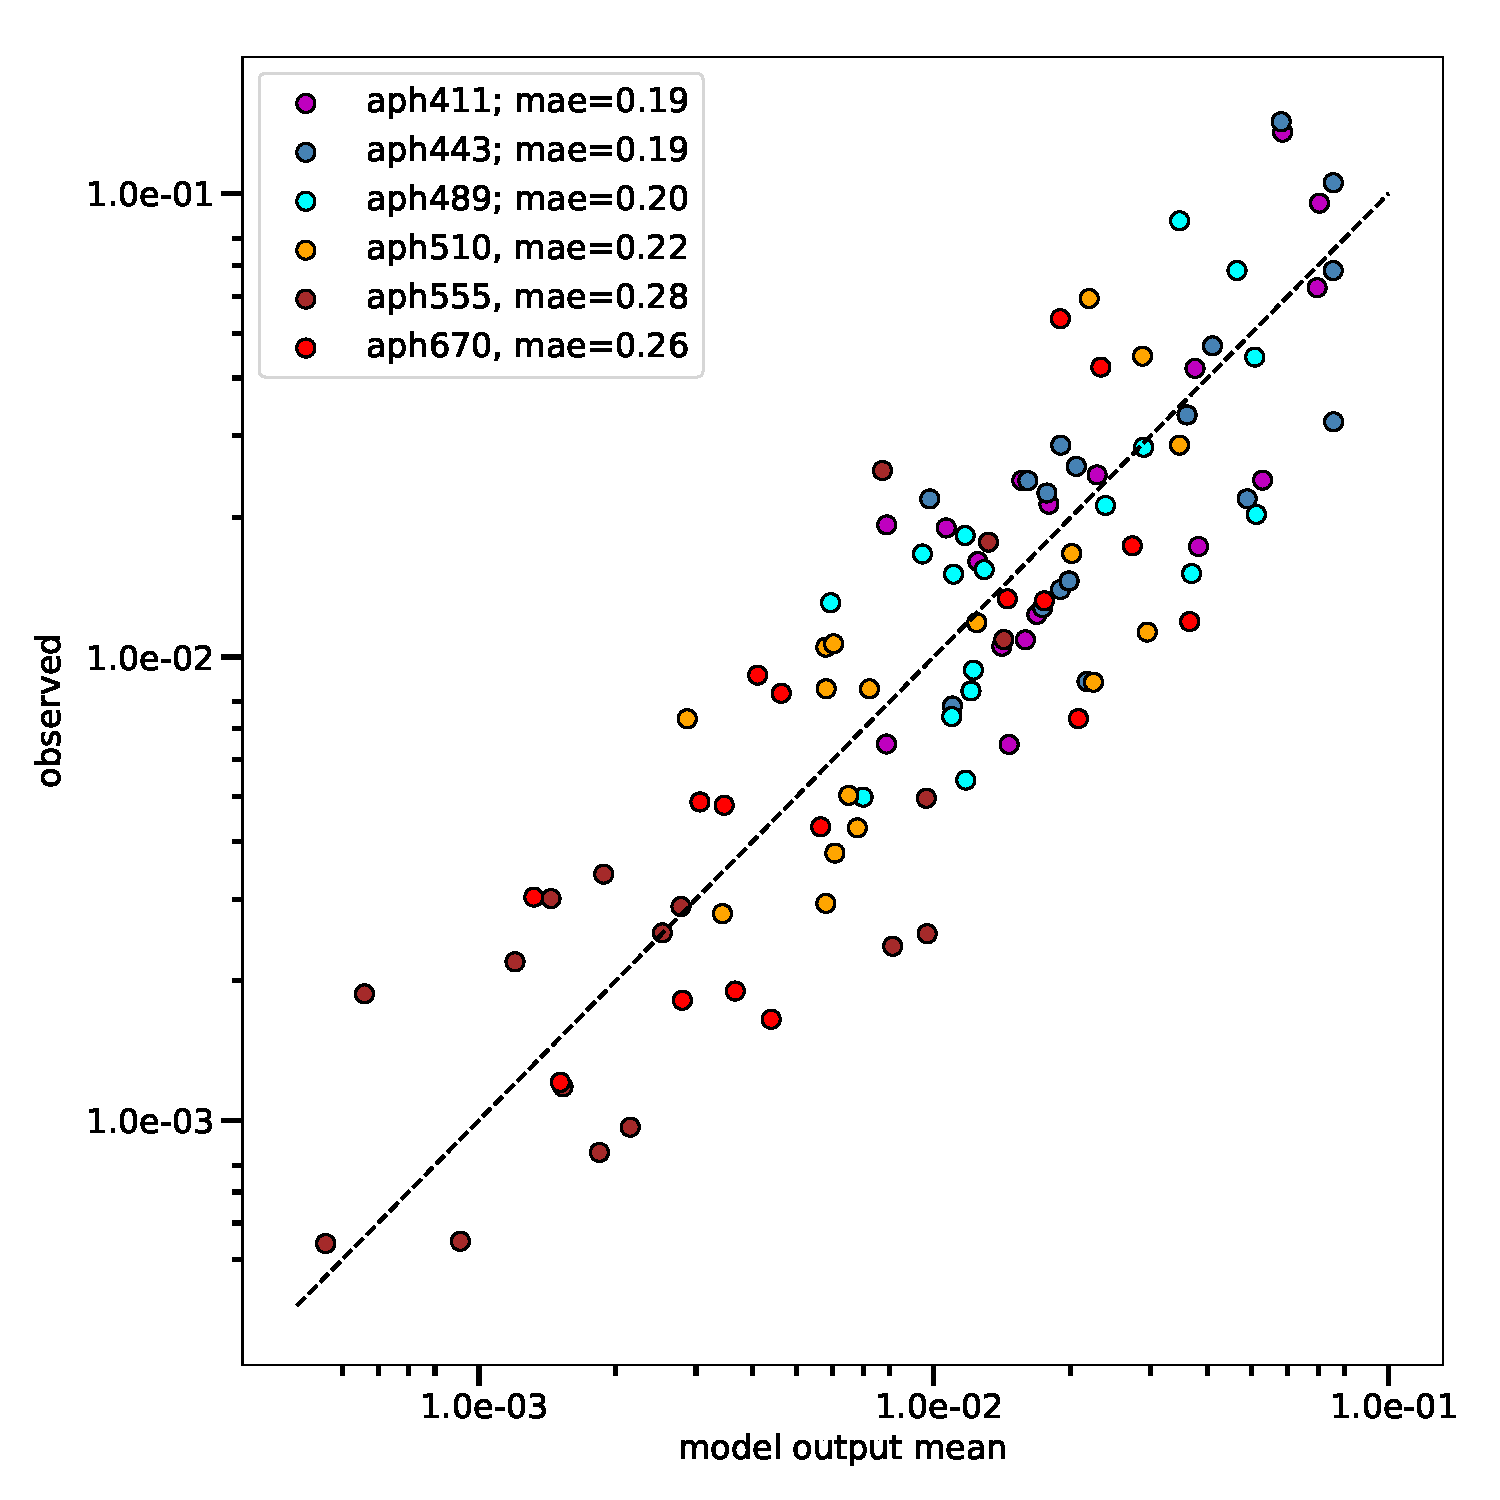
\includegraphics[height=15cm, width=0.43\columnwidth]{test_1_hs_prior_aphi_411}}
  \fbox{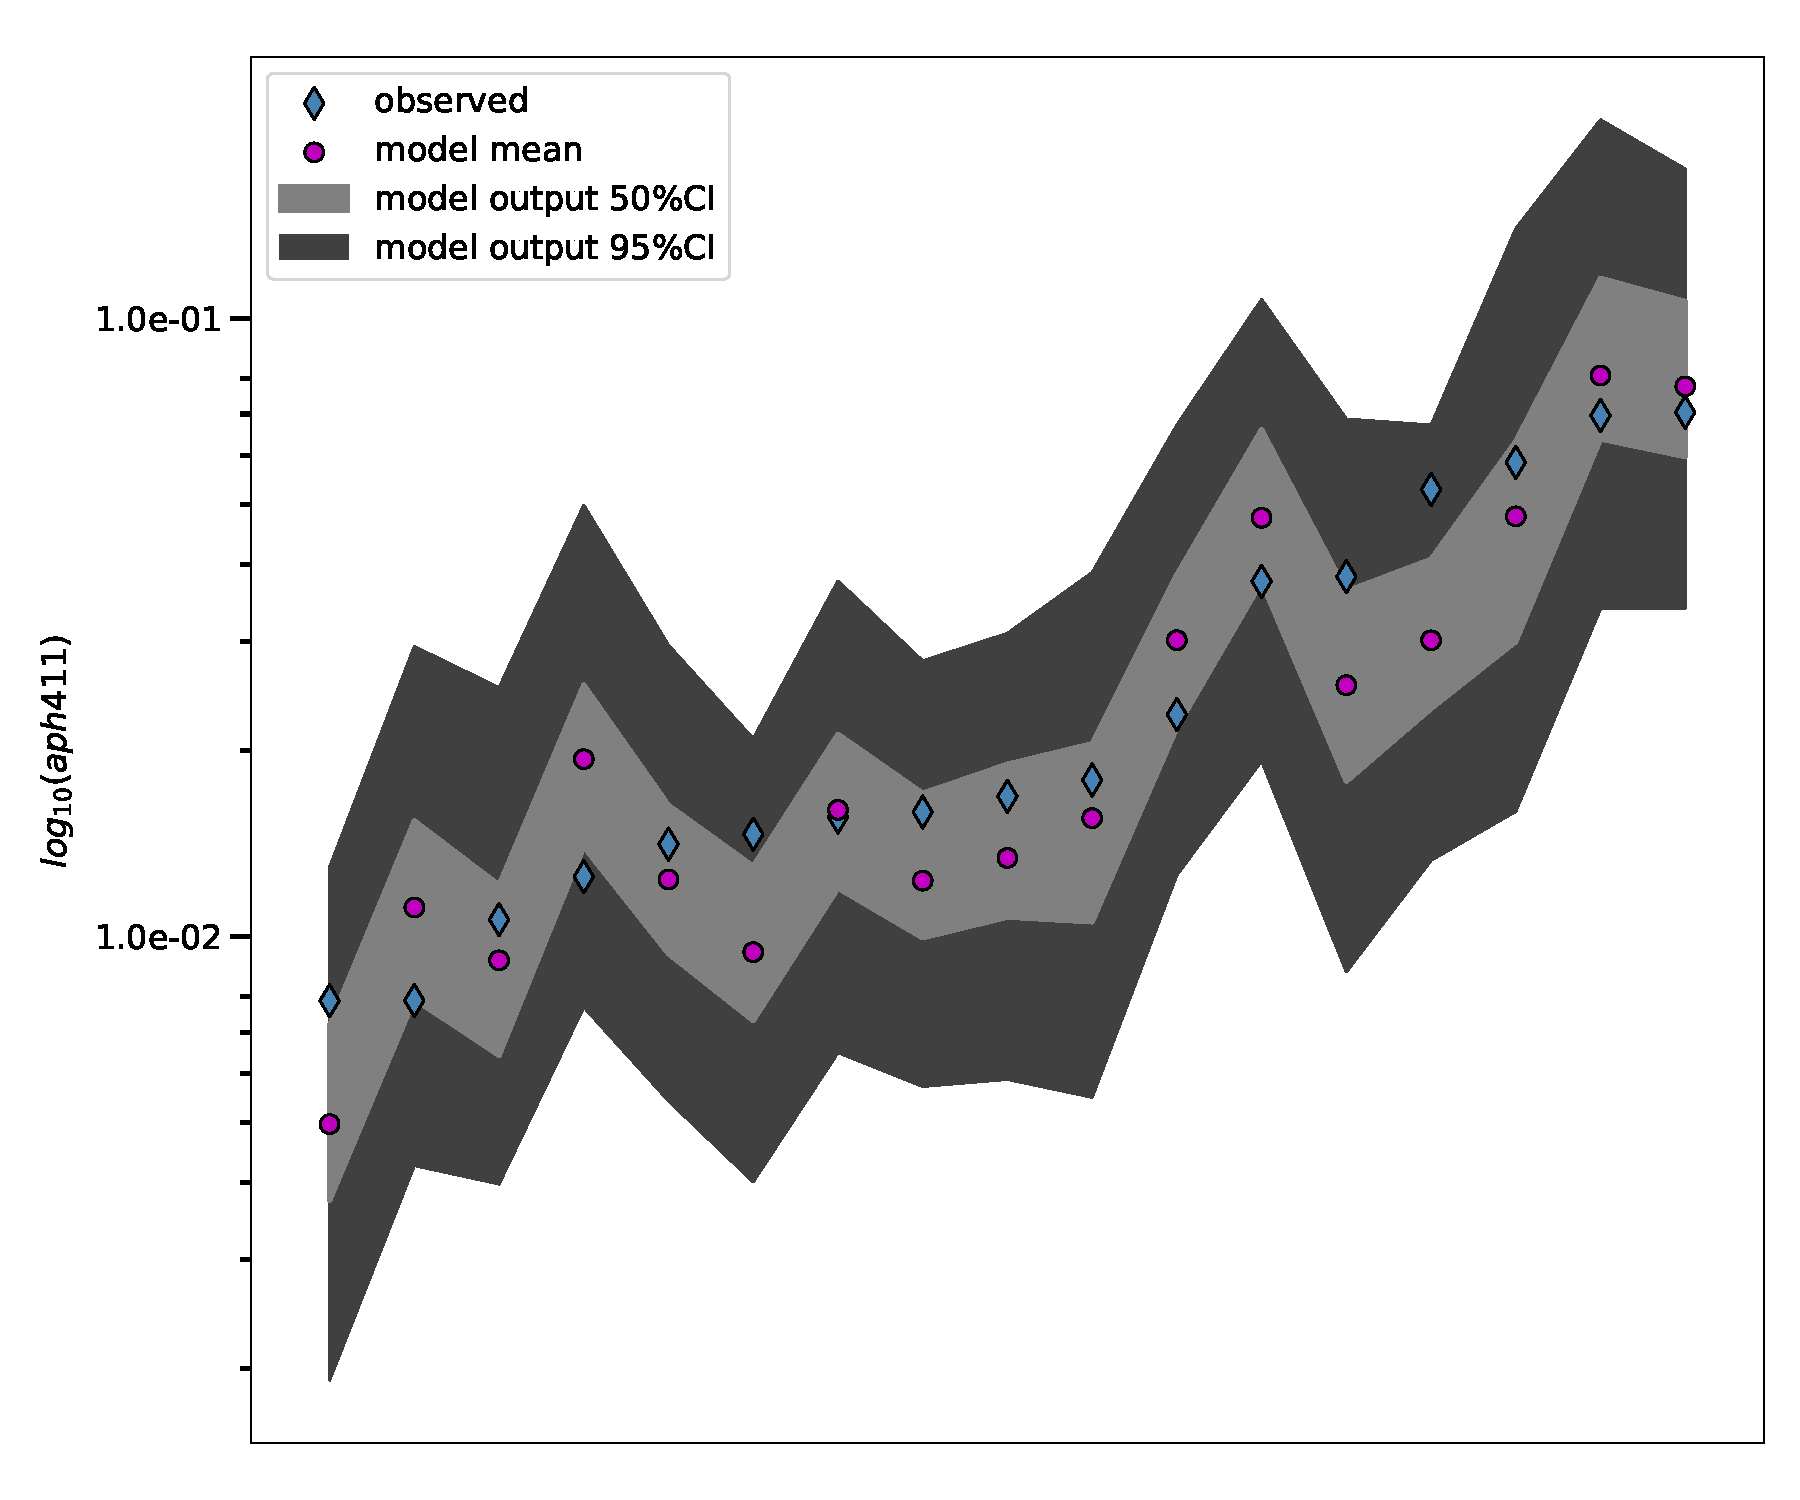
\includegraphics[height=15cm, width=0.55\columnwidth]{ppc_2_hs_wi_aphi_411}
  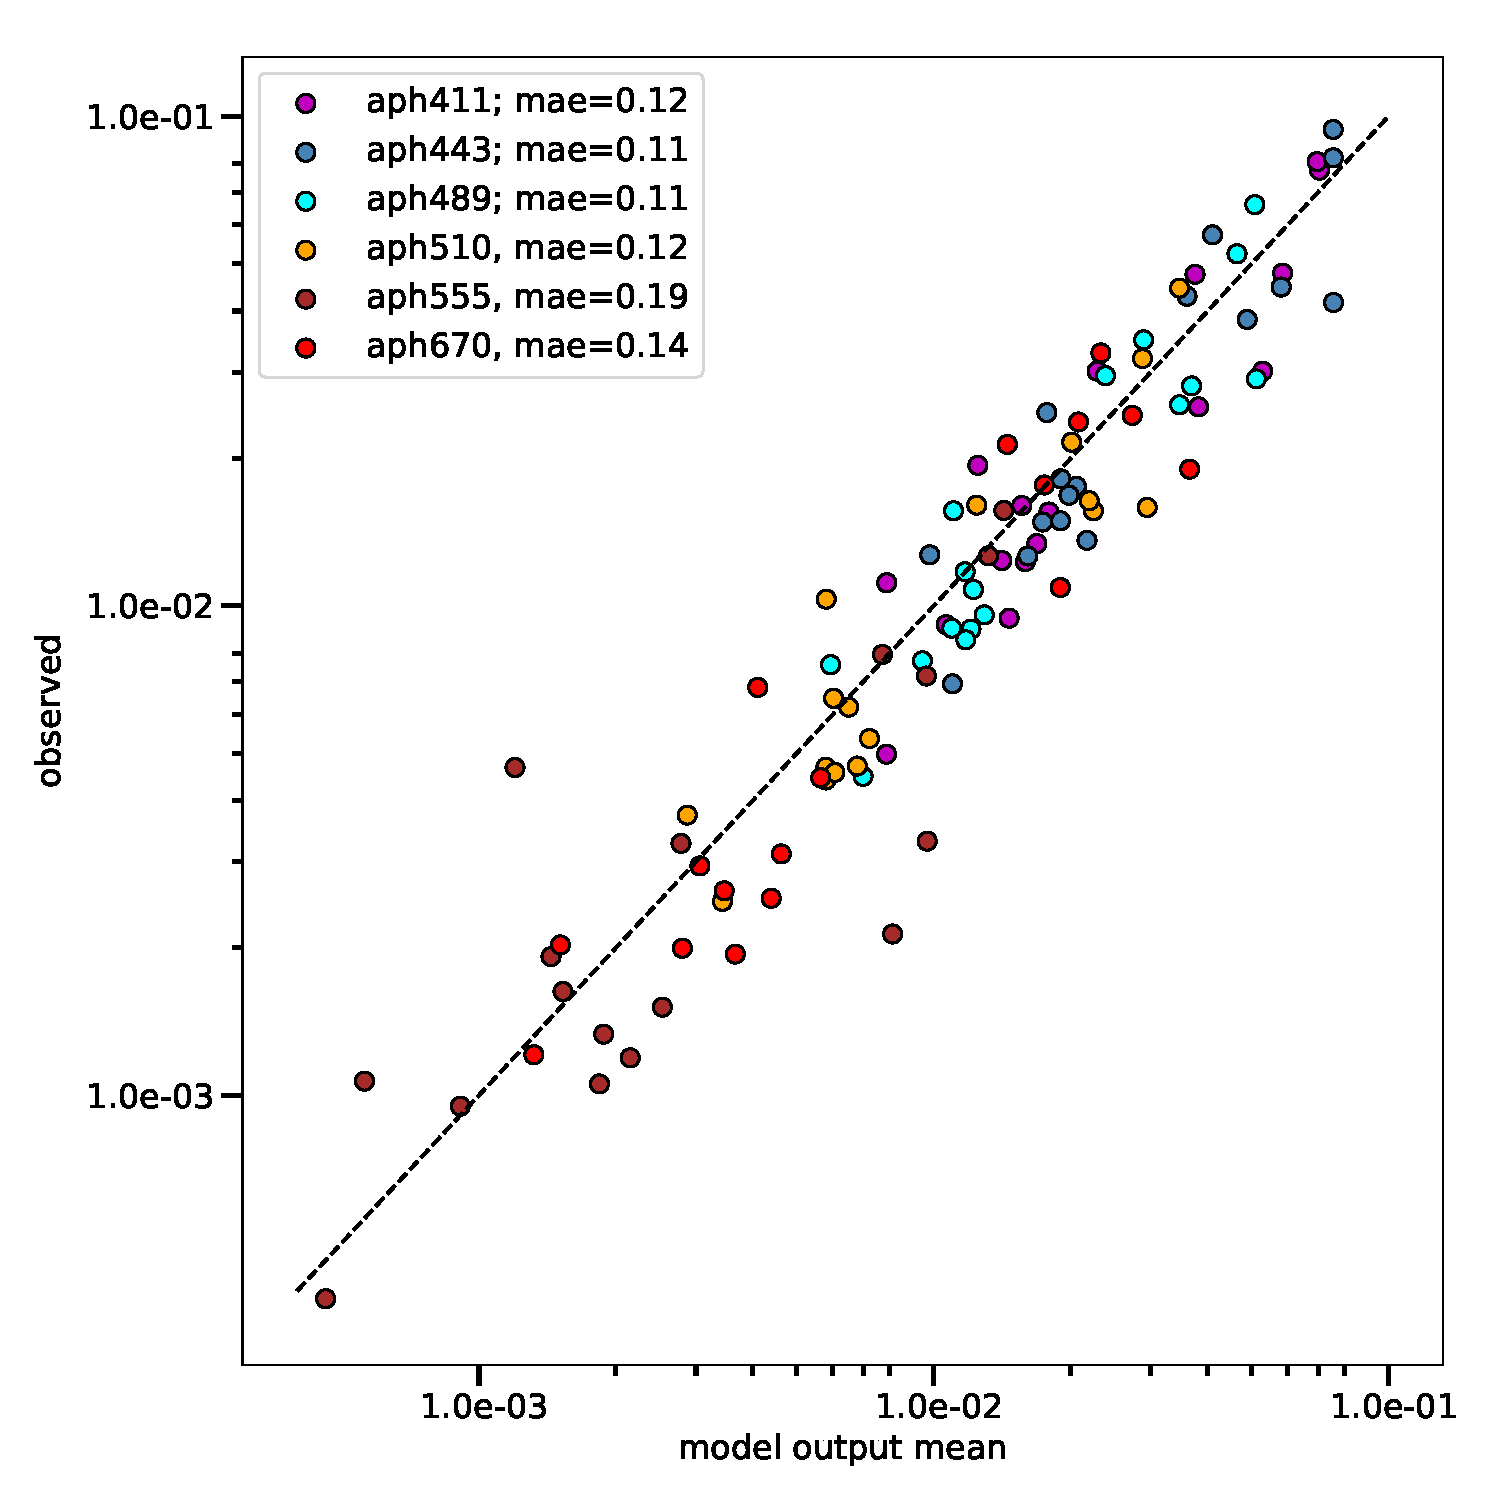
\includegraphics[height=15cm, width=0.43\columnwidth]{test_2_hs_prior_wi_aphi_411}}
  \fbox{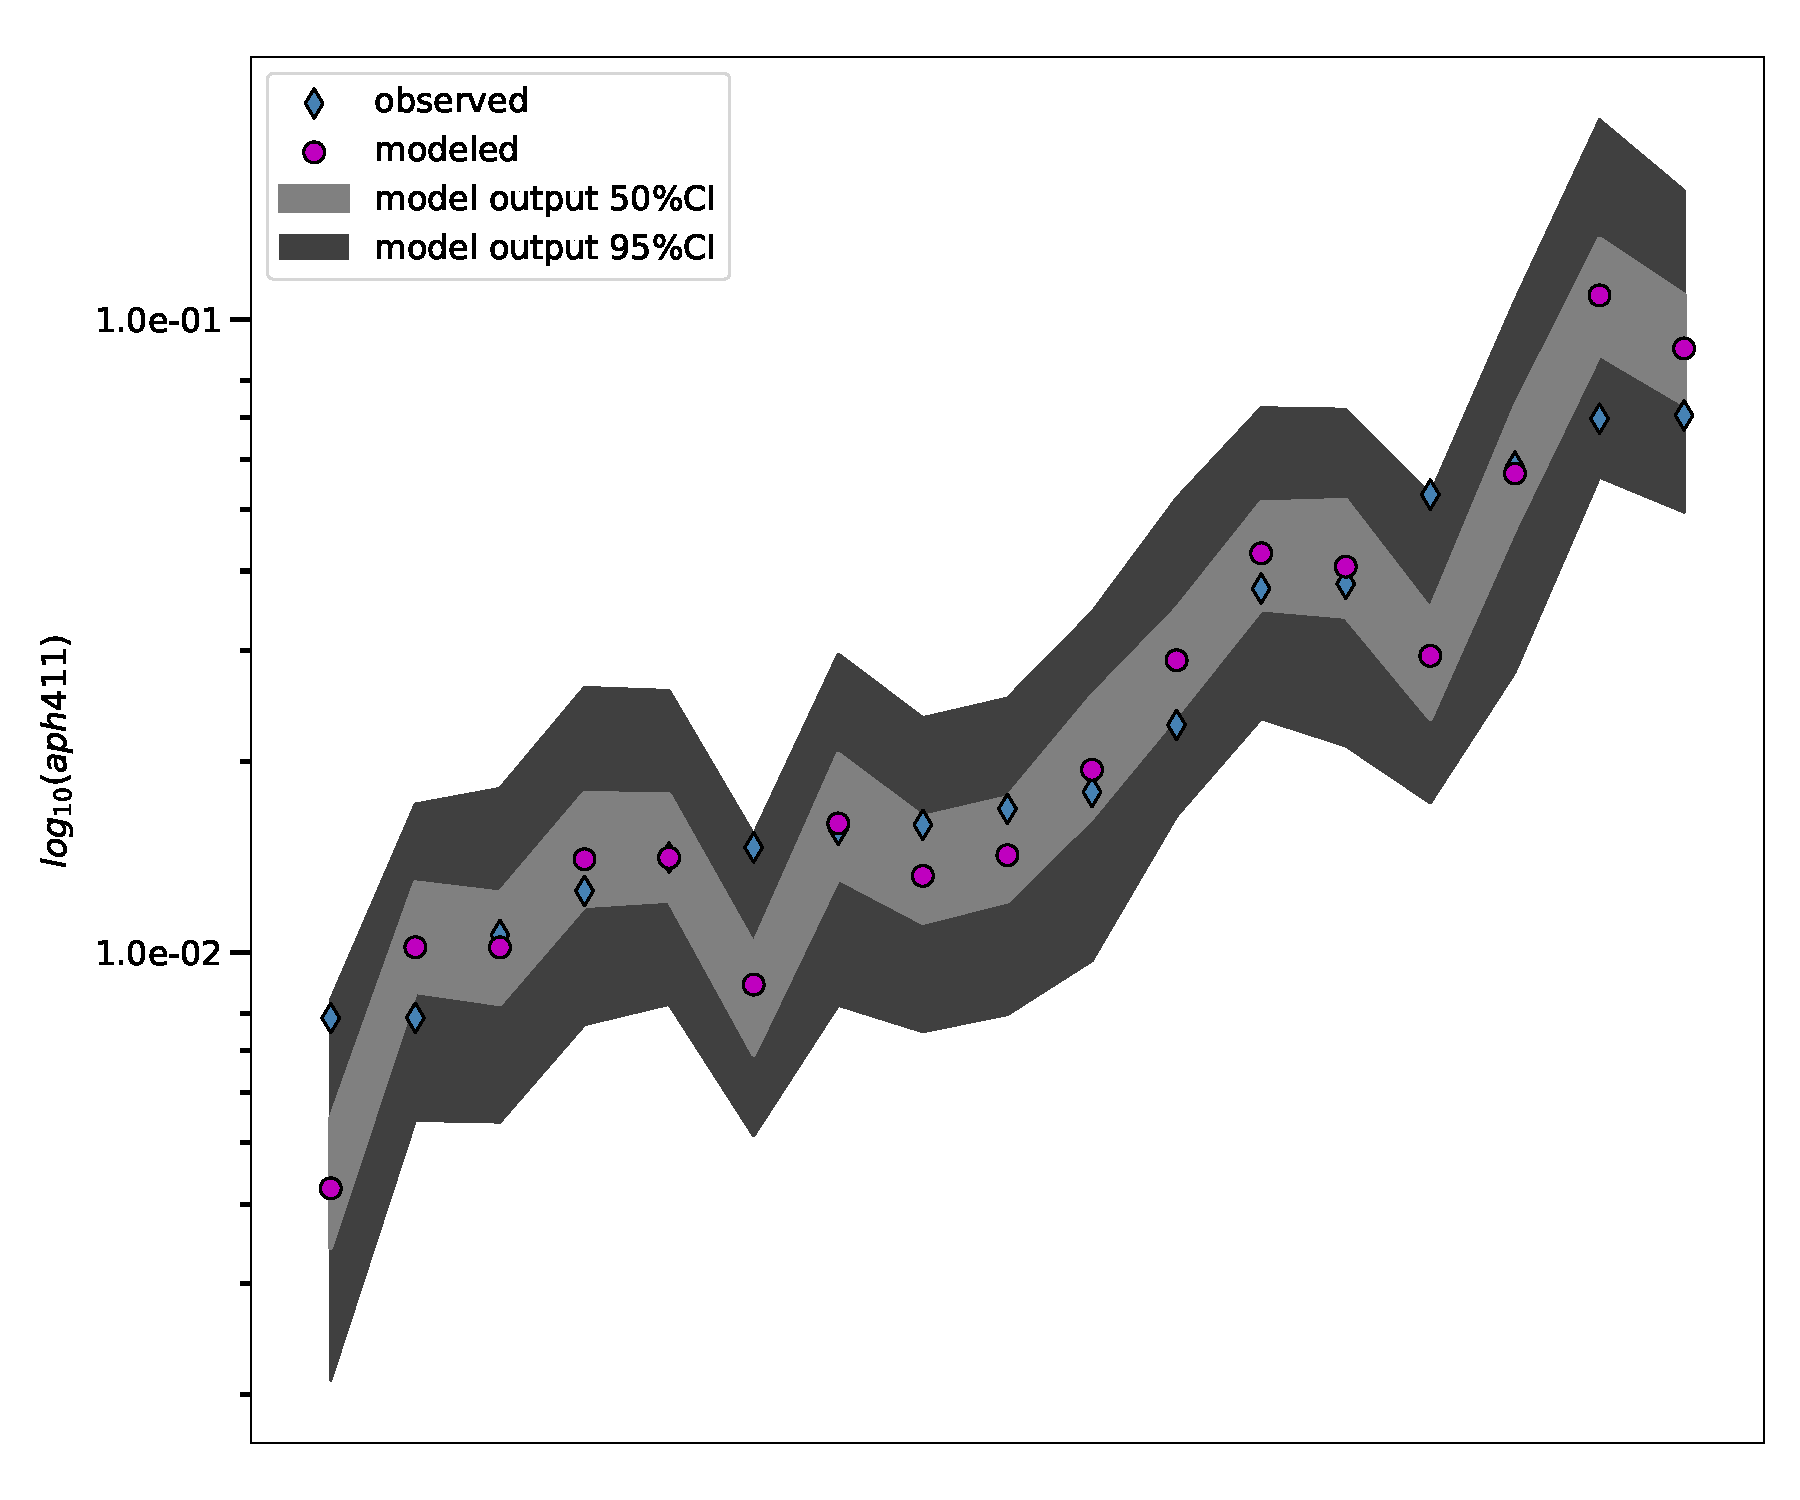
\includegraphics[height=15cm, width=0.55\columnwidth]{ppc_3_bnn_aphi_411}
  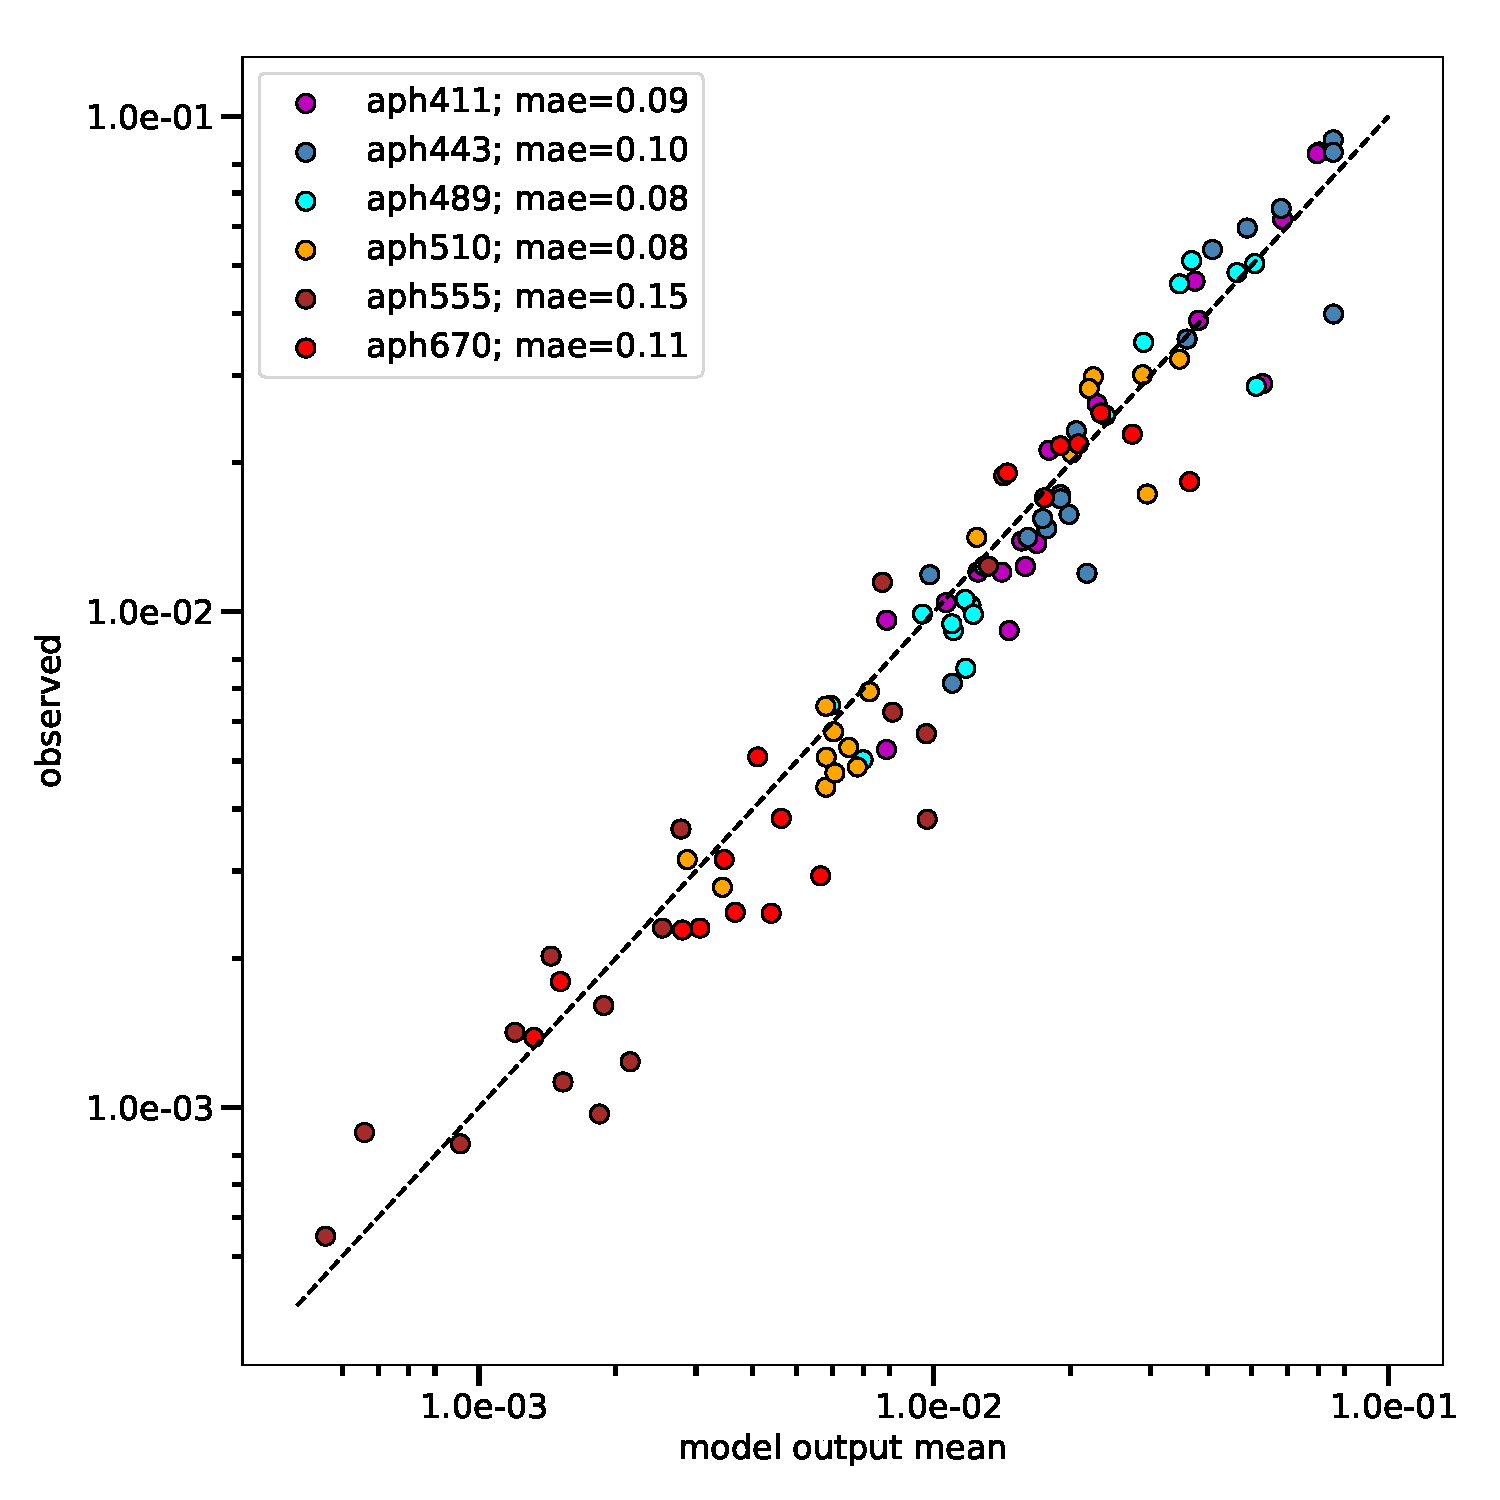
\includegraphics[height=15cm, width=0.43\columnwidth]{test_3_bnn_aphi_411}}
  \captionof{figure}{Top, middle and bottom panels correspond to Models 1, 2, and 3, respectively. \textbf{Left} plot shows out-of-sample  observations of \textbf{aph} at 411nm, in relations to model posterior predictive mean, 50\%, and 95\% credibility interval, for aph at 411nm. \textbf{Right} plot shows out-of-sample against model predictions for all bands of \textbf{aph}.}
\end{center}\vspace{1cm}


\begin{center}\vspace{1cm}
\begin{tabular}{lllllll}
    \toprule
    {} &    WAIC & pWAIC &   dWAIC & weight &     SE &    dSE \\
    \midrule
    \textbf{Model 3} & \textbf{-183.21} &    \textbf{29} &       \textbf{0} &   \textbf{0.98} &  \textbf{21.51} &      \textbf{0} \\
    Model 2 &  -70.48 &  32.7 &  112.72 &      0 &  18.49 &  16.09 \\
    Model 1 &  -25.91 &  9.81 &   157.3 &   0.02 &  15.01 &  19.93 \\
    \bottomrule
    \end{tabular}
    \captionof{table}{\textbf{W}idely \textbf{A}vailable \textbf{I}nformation Criterion for models predicting \textbf{aph} at 411 nm. WAIC takes into account model complexity and the posterior distribution of a model to predict its performance on future (out-of-sample) data. \textbf{WAIC}: lower score predicts better performance; \textbf{pWAIC}: effective number of parameters - a measure of model flexibility ; \textbf{dWAIC}: difference with lowest WAIC ;\textbf{weight}: can be used when ensemble averaging similarly scored models when no clear winner is available; \textbf{SE}: standard error of WAIC estimate ; \textbf{dSE}: standard error of dWAIC. Here, \textbf{Model 3}, the Bayesian Neural Network model is predicted to be a more robust model, and proposed as sole model to be selected.}
    \end{center}
%----------------------------------------------------------------------------------------
%	CONCLUSIONS
%----------------------------------------------------------------------------------------

\color{SaddleBrown} % SaddleBrown color for the conclusions to make them stand out

\section*{Conclusions}

\begin{itemize}
    \item Bayesian inference provides a principled modeling framework.
    \item Assumptions are explicit resulting in criticizable models that can be built to be comparable.
    \item By all measures, \textbf{Model 3} is predicted to be the better performing alternative.
\end{itemize}

\color{DarkSlateGray} % Set the color back to DarkSlateGray for the rest of the content

%----------------------------------------------------------------------------------------
%	FORTHCOMING RESEARCH
%----------------------------------------------------------------------------------------

\section*{Problems and Opportunities}

The following items require attention:
\begin{itemize}
    \item Tackling symmetry issues that complicates convergence in more complicated models.
    \item Intensified in-situ data collection for better model construction.
    \item Integration of this and other approaches into existing production systems.
\end{itemize}

 %----------------------------------------------------------------------------------------
%	REFERENCES
%----------------------------------------------------------------------------------------

%\nocite{*} % Print all references regardless of whether they were cited in the poster or not
\bibliographystyle{plain} % Plain referencing style
\bibliography{bayes} 


%----------------------------------------------------------------------------------------

\end{multicols}
\end{document}